% !TeX root = ../main.tex

\chapter{分支融合的部署方法}

\section{引言}

近年来,深度学习快速发展,已在许多任务中达到了优异的性能表现,使其越来越多的应用在众多生活与工业领域。但这些深度神经网络模型优异的性能都依赖于具有数百万甚至数十亿个参数的深度网络模型,需要消耗大量的计算资源和存储资源,需要高性能的硬件作为支撑,这对实际部署、运行和应用的环境提出了较高的要求。因此,深度神经网络的压缩与优化一直都是一个非常关键的问题,特别是对于计算资源有限的嵌入式移动设备来说,如此高的计算资源要求是不可接受的。另一个关键的挑战是能源消耗:由于移动设备的电池有限,繁重的计算会很快耗尽电池。然而大多数的模型压缩算法与高效的网络结构对于计算硬件并不友好,虽然能够显著模型参数,但是并没有很好的利用硬件性能,达到理论的上的加速比。

目前大多数的模型压缩与轻量化研究,都是力图用更少的参数和更快的计算得到与大规模网络模型一致或差不多的模型精度,并没有考虑到模型训练时和部署时的差异性。模型训练要求模型精度,训练速度;而模型部署则要求模型在部署端的硬件高效性、内存高效性和运行效率。

模型的压缩与轻量化研究,终究是为了提高模型的参数效率与运行效率,力图用更少的参数和更快的计算得到与大规模网络模型一致或差不多的模型精度。反过来,如果在同样的参数和计算量的前提下,能够显著提升模型的精度表现或加快模型推理速度,也是同样达到的提高模型参数效率和运行效率的目的。特别是对于资源固定的嵌入式设备,如果能够优化符合设备资源要求的尽量大的网络模型的推理精度和推理效率,这将是模型优化在另一种思路的解决办法。在保持网络性能的前提下,持续缩小网络参数并不是一个容易的目标,目前大多数的研究也正是将其作为研究目标,比如模型裁剪,模型量化,矩阵/张量低秩分解等等。换个角度,在保持模型参数和计算规模不变的前提,提高模型推理精度和推理速度也是一个模型优化的方法。现阶段大多数这方面的研究都集中在优化深度学习框架和模型部署工具方面,通过提高模型并行度,减少参数访存和模型在特定硬件的计算效率等加快模型推理速度。

在任意深度学习的应用场景落地一个模型/算法时,需要经历两个基本步骤:
\begin{itemize}
    %\vspace{-1em}
    \item[1)] 根据数据生产一个模型的训练步骤;
    \item[2)] 将生产出的模型部署到目标设备上执行服务的推理步骤。
\end{itemize}

训练步骤目前基本由Tensorflow \cite{tensorflow}、PyTorch \cite{pytorch}、MXNet \cite{mxnet} 等主流框架主导,但是在部署步骤,基本是处在“百家争鸣”的状态,不同的部署框架对于不同的硬件架构有着专门的手动优化,在相应平台能够实现更快的运行速度,比如NCNN \cite{ncnn} 针对手机移动端做了专门的优化,TensorRT \cite{tensorrt} 针对NVIDIA GPU架构,特别是其嵌入式深度学习设备进行专门的优化和部署,运行效率和资源消耗都远远低于 Pytorch 等通用框架,同时高通和苹果也都发布了针对自家平台优化的深度学习部署框架。

严格来说部署工具的优化并不通用,也并不是针对网络模型方面的优化,最近开始有相关研究开始研究模型部署使得性能优化 \cite{ding2019acnet, ding2021repvgg, ding2021diverse},本章也从这个角度入手,提出分支融合部署方法,针对类 \cite{he2016deep} 网络,通过融合多分支结构,在不损失精度的前提下进行结构替换和融合,提高模型部署时的运行效率。

本章首先介绍相关新兴研究方向,之后进行分析多分支网络结构和线性网络结构的特点,进而引出本章提出的分支融合部署方法,之后详细介绍采用重参数化和知识蒸馏进行分支融合的原理与方法,最后对本章进行总结。

\section{重参数化与辅助训练}

重参数化是指,模型训练阶段和模型推理阶段分别使用不同的网络结构和模型参数,在模型训练完成之后通过结构和参数变换,将训练阶段的模型参数和结构转变成推理阶段使用的参数和结构,即模型的训练阶段和模型的推理阶段的行为并不完全一致。其中,模型结构和参数变换的约束条件是是它们所表示的模型功能在数学上是等价的。一般来说,进行重参数化是为了在模型训练阶段能够达到更高的精度,在推理阶段能够更加高效的运行。即训练阶段倾向于易于优化,推理阶段倾向于高效部署。从这个角度来看,批归一化BatchNomalization \cite{ioffe2015batch}的工作也可以看作是重参数化的一个代表,Nvidia TensorRT \cite{tensorrt} 在部署时采用的网络融合也是重参数化的应用,近期丁等人提出ACNet \cite{ding2019acnet},使用1*3和3*1非对称卷积在训练时提升3*3卷积的性能,在部署时将其融合为1个3*3卷积,实现无代价的性能提升,RepVGG \cite{ding2021repvgg} 提出在原始VGG网络基础上引入1x1卷积和identity辅助分支来解决模型优化问题,最终在部署时融合为纯3*3卷积的线性网络,获得在速度和精度两方面的性能提升。Diverse Branch Block \cite{ding2021diverse} 提出了一个通用的类似于Inception Block的结构来替换普通的卷积,极大地丰富模型的微观结构,提升多种架构的性能,这样一个复杂的block可以在训练结束后等价转换为一个卷积,因此模型的最终大小和速度(相对于使用普通卷积的模型)完全不变。

辅助监督在训练时使用额外的辅助损失函数来得到更高的性能,辅助损失函数只在训练时存在,在部署时舍弃。LabelEnc \cite{hao2020labelenc} 提出在训练时采用额外结构LabelEncoding Function对网络中间特征进行监督,利用类似模型蒸馏的方法完整训练检测模型,并在推理时舍弃额外结构实现无痛涨点。

重参数化和辅助监督这两个思路的共同特性是只是训练阶段使用的技巧而不增加推理阶段的开销,实现模型推理精度的提升,因此它们在实际模型训练过程和部署过程是非常有利的。

\section{线性网络与多分支结构网络}

\subsection{线性网络}

卷积神经网络最早由LeCun提出,首个卷积神经网络LeNet[]和早期卷积神经网络AlexNet[]、VGGNet[]等都是朴素的线性结构,即层与层之间以此前后连接起来,没有跳层连接和分支,一个典型的线性网络代表就是VGGNet,形如图~\ref{fig:vgg16_}。VGGNet是ILSVRC 2014上的相关工作,取得了当年图像定位的冠军,在ImageNet数据及上获得了68.5 \% 的Top1精度和88.7 \% 的Top5精度。其主要工作是证明了增加卷积神经网络的深度能有效提高模型精度,并且多次使用小卷积核可以获得更大的感受野,等效于直接使用大卷积核,如2个3*3卷积核相当于1个5*5卷积核、3个3*3卷积核相当于1个7*7卷积核,同时能够有效减少参数。如图~\ref{fig:vgg16}所示,VGG包含5层卷积结构、3层全连接层、softmax输出层,层与层之间使用max-pooling(最大池化)缩小尺寸,采用ReLU激活函数。VGG有两种结构,分别是VGG-16和VGG-19,两者除了网络深度不一样并没有本质上的区别。

\begin{figure}[]
    \centering
    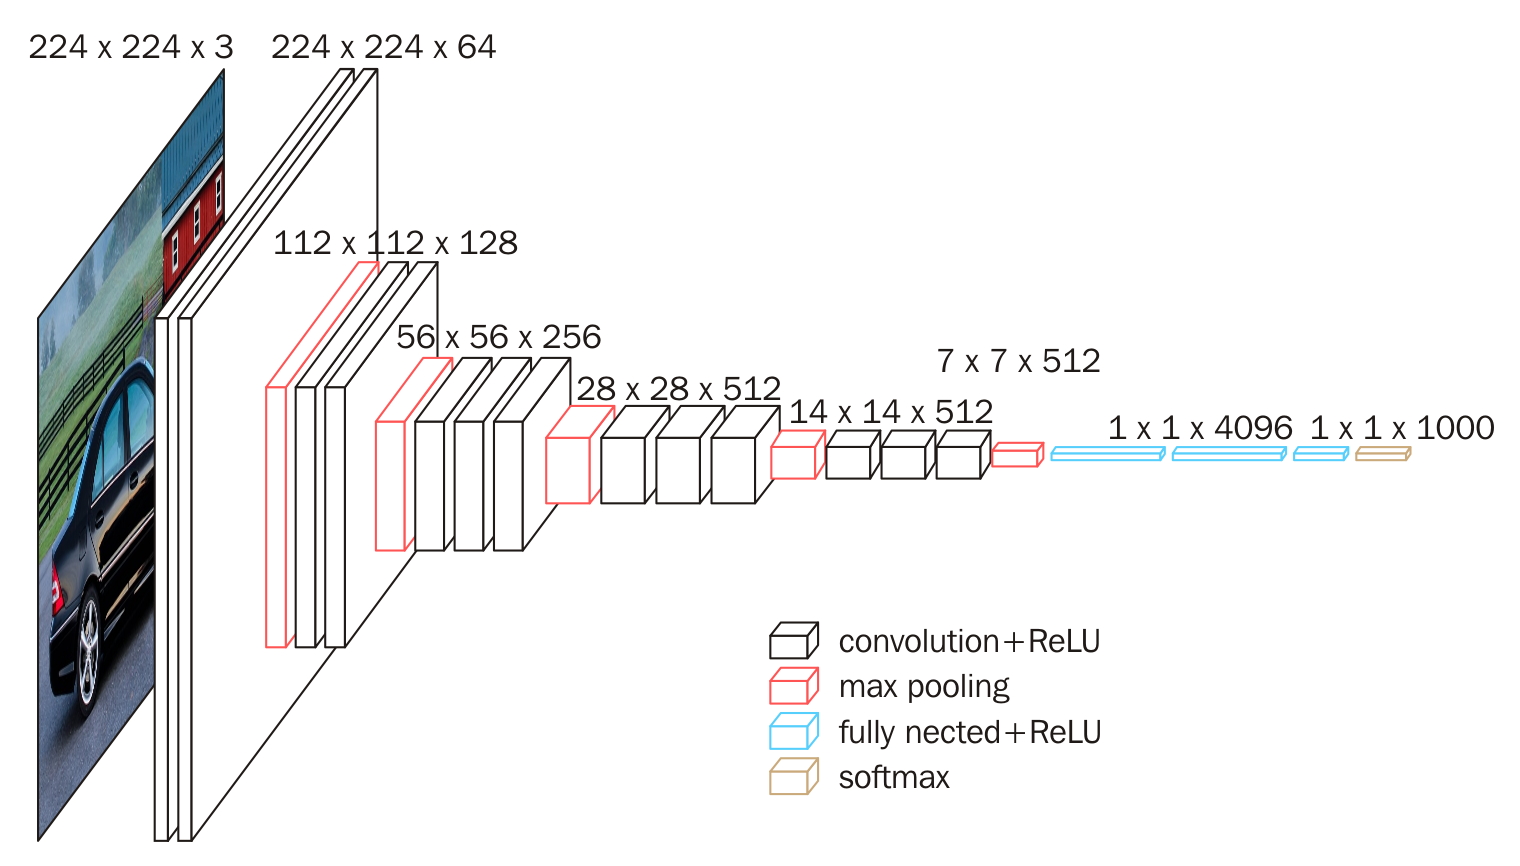
\includegraphics[width=1\textwidth]{vgg16.png}	%\vspace{-1.0em}
    \caption{VGG-16,线性网络结构}
    \label{fig:vgg16_} %\vspace{-0.8em}
\end{figure}

\subsection{残差模块与shortcut连接}

残差模块与shortcut连接由ResNet提出[],使用shortcut跳层连接,可以训练更深的神经网络。ResNet的结构如图~\ref{fig:resnet_}所示。ResNet(残差神经网络)是由微软研究院的何恺明等人提出的。残差神经网络的主要贡献是发现了“退化现象(Degradation)”,并针对退化现象发明了Shortcut,提出了带有旁路层的残差模块,帮助梯度在层与层之间能够更加容易的传递,解决了深度过大的神经网络训练困难的问题,使得神经网络的“深度”首次突破了100层,最大甚至可以超过1000层。

\begin{figure}[]
    \centering
    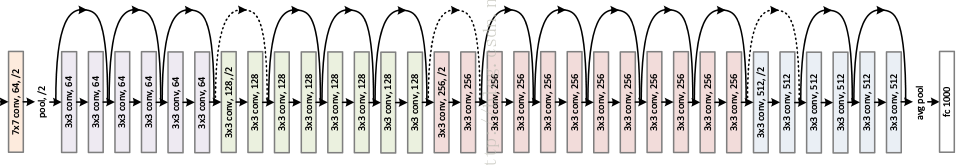
\includegraphics[width=1\textwidth]{resnet.png}	%\vspace{-1.0em}
    \caption{ResNet,残差网络结构}
    \label{fig:resnet_} %\vspace{-0.8em}
\end{figure}

ResNet使用两种不同的残差单元,如图~\ref{fig:residual}所示。左图对应的是浅层网络的残差结构,而右图对应的是深层网络的残差结构。对于短路连接,当输入和输出维度一致时,可以直接将输入加到输出上。但是当维度不一致时,这就不能直接相加。有两种策略:(1)采用zero-padding增加维度,此时一般要先做一个downsamp,可以采用strde=2的pooling,这样不会增加参数;(2)一般采用1x1的卷积(projection shortcut),这样会增加参数,也会增加计算量。短路连接除了直接使用恒等映射,也可以采用1x1卷积。

\begin{figure}[]
    \centering
    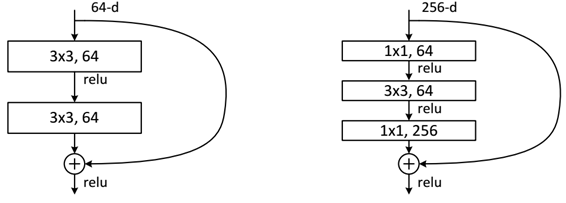
\includegraphics[width=1\textwidth]{residual.png}	%\vspace{-1.0em}
    \caption{两种的残差结构}
    \label{fig:residual} %\vspace{-0.8em}
\end{figure}


\subsection{多分支inception模块}

GoogleNet使用inception模块作为其卷积的基本单元,inception模块是一种多分支和多尺度的卷积核拼接而成。如图~\ref{fig:googlenet_}所示,GoogleNet即Inception-V1,它以inception单元为基本结构,具有9个inception模块,每个inception模块由四个分支组成,分别是1×1、3×3、5×5卷积和down-sampling,具有多尺度感受野。inception结构的主要贡献有两个:一是使用1x1的卷积来进行升降维;二是使用多尺度的卷积核进行特征提取。训练时使用两个辅助损耗层从中间层注入Loss,防止梯度消失,而在推理时,删除辅助层。

\begin{figure}[]
    \centering
    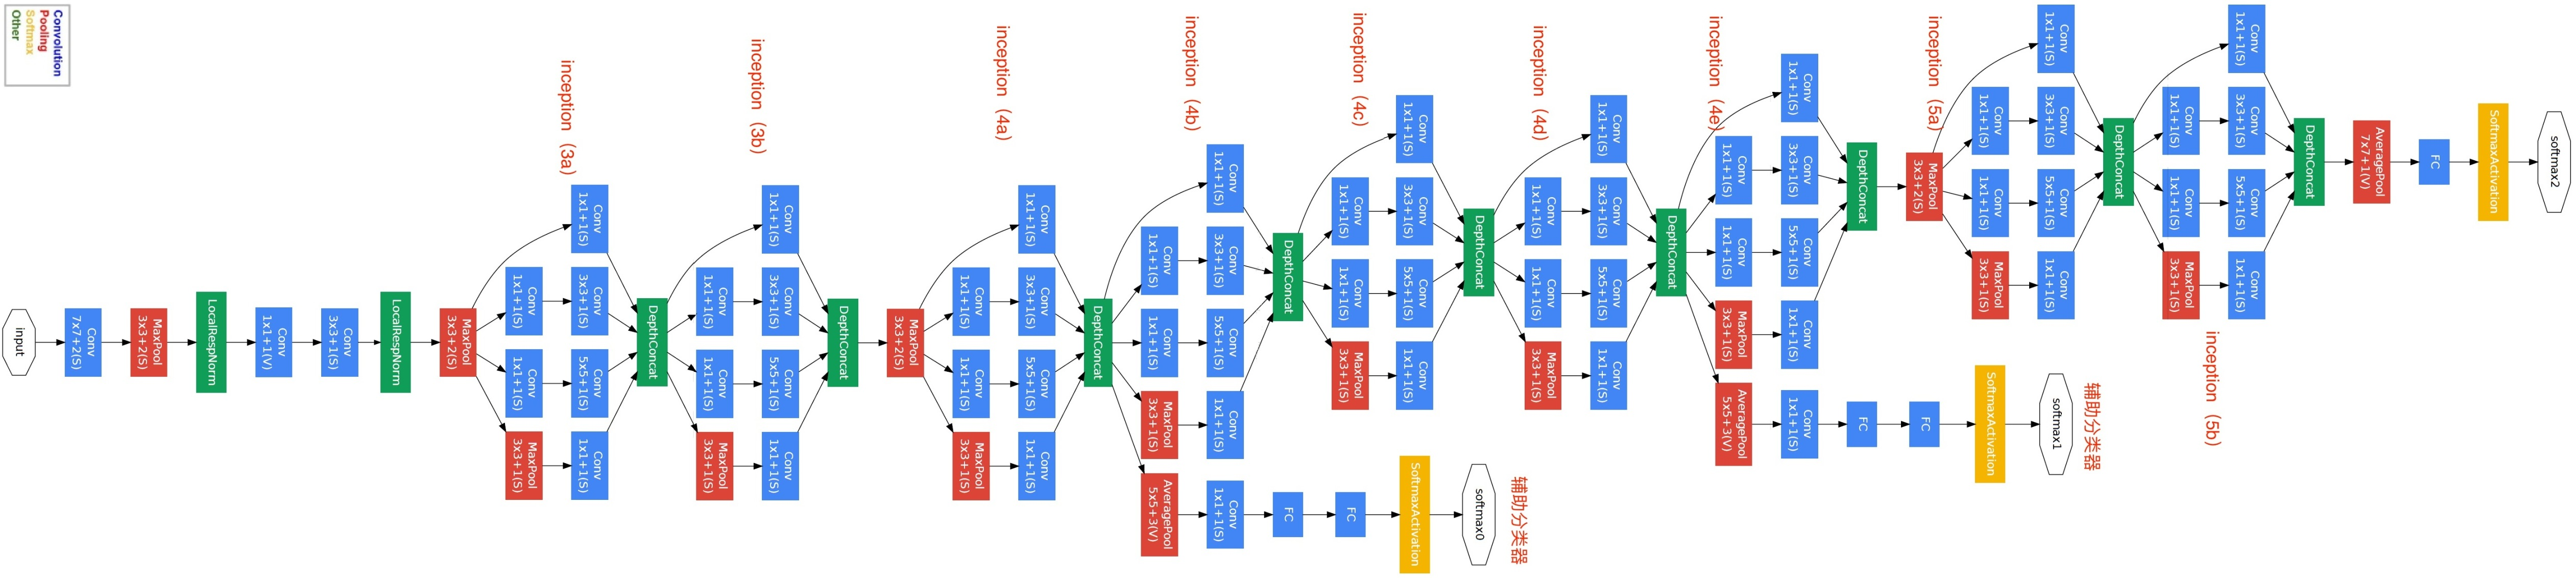
\includegraphics[width=1\textwidth]{googlenet.jpg}	%\vspace{-1.0em}
    \caption{GoogleNet,多分支inception模块}
    \label{fig:googlenet_} %\vspace{-0.8em}
\end{figure}

残差结构经过发展,有多种变形,但其主要思想就是通过在多分支上进行多尺度的卷积运算,在多个感受野上进行特征提取,为了减少计算量,使用两个3*3卷积代替5*5,使用1*7和7*1卷积代替7*7卷积。

\begin{figure}[]
    \centering
    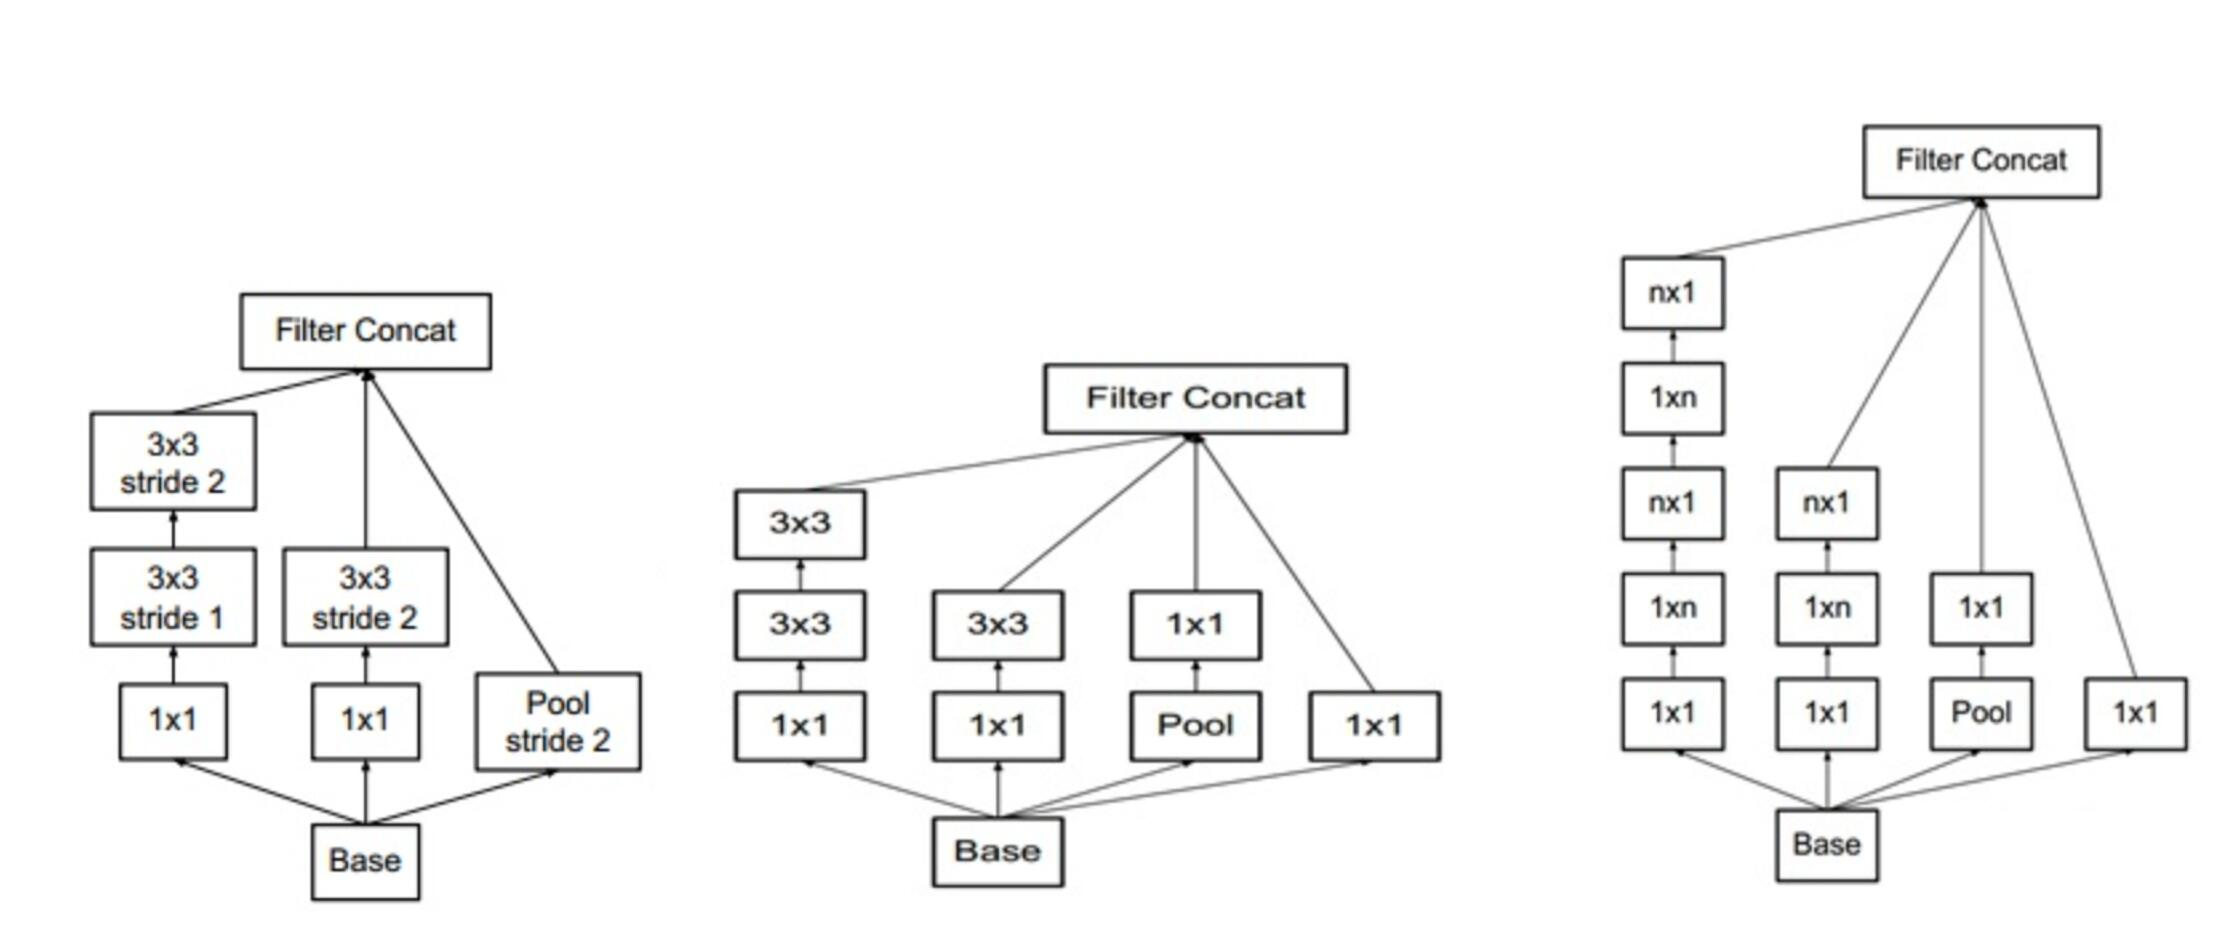
\includegraphics[width=1\textwidth]{inception.jpg}	%\vspace{-1.0em}
    \caption{3种的残差结构}
    \label{fig:inception} %\vspace{-0.8em}
\end{figure}

\subsection{线性网络与多分支网络对比}

多分支网络结构如,残差模块通过shortcut快捷连接,直接将训练损失回传,避免了深层神经网络的退化问题,可以训练更深的网络;inception模块利用多分支卷积,通过合并多个感受野下的特征使得网络训练性能更好。它们都能提升网络参数的表达能力,对与网络训练是有意义的。但是,相比于单路结构,多分支结构对内存不友好,同时不利于并行化,并不能完全利用计算和内存资源。如图~\ref{fig:plain_res}所示,具有分支的结构会保存之前计算的特征图,在add或cat之前都需要常驻内存,对内存不友好。他们的优缺点如表\ref{tab:plain_res}所示,可以看到,多分支网络训练友好部署不友好,线性网络则恰好相反。

\begin{figure}[]
    \centering
    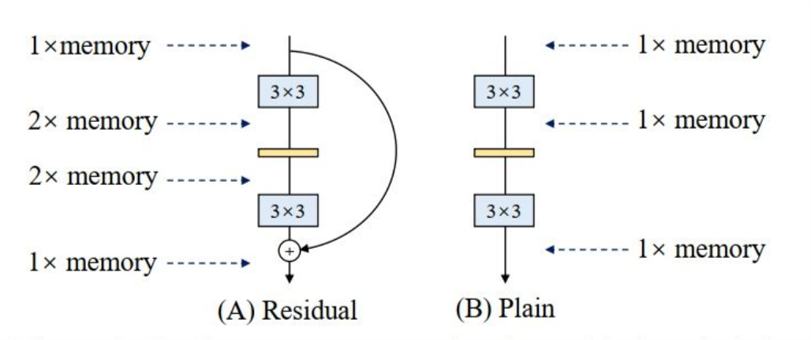
\includegraphics[width=1\textwidth]{plain_res.png}	%\vspace{-1.0em}
    \caption{残差结构与线性网络内存使用对比}
    \label{fig:plain_res} %\vspace{-0.8em}
\end{figure}

\begin{table}[]
    \centering
    \caption{线性网络与多分支网络优缺点}
    \label{tab:plain_res} %\vspace{-0.8em}
    \begin{tabular}{lll}
    \hline
    网络类型  & 优点                                                              & 缺点                                                      \\ \hline
    线性网络  & \begin{tabular}[c]{@{}l@{}}并行度高\\ 内存效率高\\ 推理速度更快\end{tabular}   & \begin{tabular}[c]{@{}l@{}}不利于反向传播\\ 训练不友好\end{tabular} \\ \hline
    多分支网络 & \begin{tabular}[c]{@{}l@{}}利于反向传播\\ 多尺度感受野\\ 参数效率高\end{tabular} & \begin{tabular}[c]{@{}l@{}}不利于并行\\ 内存效率低\end{tabular}   \\ \hline
    \end{tabular}
\end{table}

\section{多分支卷积核融合}

相比于各种多分支架构(如ResNet,Inception,DenseNet,各种NAS架构等),近年来VGG式的线性网络模型鲜有关注,主要自然是因为性能差。例如,有研究[1]认为,ResNet性能好的一种解释是ResNet的分支结构(shortcut)产生了一个大量子模型的隐式ensemble(因为每遇到一次分支,总的路径就变成两倍),单路架构显然不具备这种特点。既然多分支架构是对训练有益的,而我们想要部署的模型是单路架构,我们提出解耦训练时和推理时架构,将网络模型的训练和部署区分,流程如下:

\begin{itemize}
    %\vspace{-1em}
    \item[1)] 训练一个多分支网络模型
    \item[2)] 将多分支模型进行分支融合,尽量等价转换为单路模型
    \item[3)] 部署融合后模型
\end{itemize}

这样就可以同时利用多分支模型训练时的优势(性能高)和单路模型推理时的好处(速度快、省内存)。这里的关键显然在于这种多分支模型的构造形式和转换的方式。

在这里,我们需要对残差结构进行一定修改,如图~\ref{fig:res-fuse}所示,在训练时,为对未下采样的残差结构每一个3x3卷积层添加平行的1x1卷积分支和identify分支,对于下采样的残差结构则少一个identify分支,确保能够在训练之后通过代数运算合并卷积核。

简单的卷积网络有很多优点,但有一个致命的缺点:性能差。例如,使用BN[17]等现代组件,VGG-16可以在ImageNet上达到72\%的top-1精度,这似乎过时了。我们使用重参数化方法去修改ResNet,显式地构造一个快捷分支模型信息流 $y = x + f(x)$ ,并使用一个残差学习块 $f$ 。当 $x$ 和 $f(x)$ ,当尺寸不匹配时,它变成了 $y = g(x) + f(x)$, $g(x)$ 是一个Conv1*1。ResNets成功的一个解释是,这样一个多分支架构使众多浅的模型隐式整体模型[35]。具体来说,有n个块的模型可以被解释为这2个模块的集合,因为每个块将流分支为两条路径。

\begin{figure}[]
    \centering
    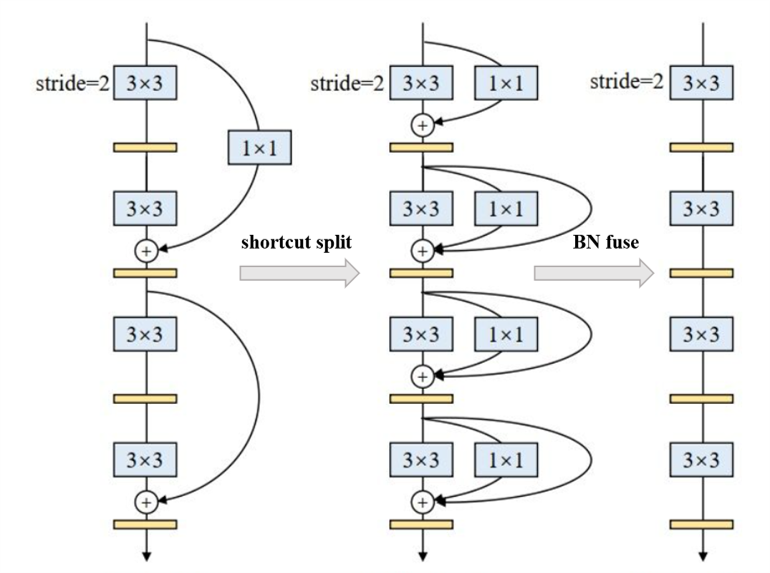
\includegraphics[width=1\textwidth]{res_fuse.png}	%\vspace{-1.0em}
    \caption{残差结构修改与分支合并}
    \label{fig:res-fuse} %\vspace{-0.8em}
\end{figure}

在训练完成后,需要对模型做等价转换,得到最终的部署模型。根据卷积的线性可加性,设三个3x3卷积核分别是 $W1$,$W2$,$W3$,则有:

\begin{equation}
    Conv(x, W1) + Conv(x, W2) + Conv(x, W3) = Conv(x, W1+W2+W3)
\end{equation}

\subsection{基于重参数化的卷积核融合}

下面将描述多种卷积核合并算法。

\subsubsection{卷积层和BN层合并}

通过合并 Conv + BN 层,减少层数,提升网络性能。

\begin{itemize}
    %\vspace{-1em}
    \item 卷积层公式为: $Conv(x) = W(x) + b$
    \item BN层公式为:$BN(x) = \gamma * \frac{x-mean}{\sqrt{var}} + \beta$
    \item 带入有: $BN(Conv(x)) = \gamma * \frac{W(x) + b - mean}{\sqrt{var}} + \beta$
    \item 化简地: $BN(Conv(x)) = \frac{\gamma * W(x)}{\sqrt{var}} + \frac{\gamma * (b - mean)}{\sqrt{var}} + \beta$
    \item 令:   $W_{fused} = \frac{\gamma * W(x)}{\sqrt{var}}$
    \item 令:   $B_{fused} = \frac{\gamma * (b - mean)}{\sqrt{var}} + \beta$
    \item 则: $BN(Conv(x)) = W_{fused} + B_{fused}$
\end{itemize}

\subsubsection{Conv3*3 和 Conv1*1合并}

\begin{figure}[]
    \centering
    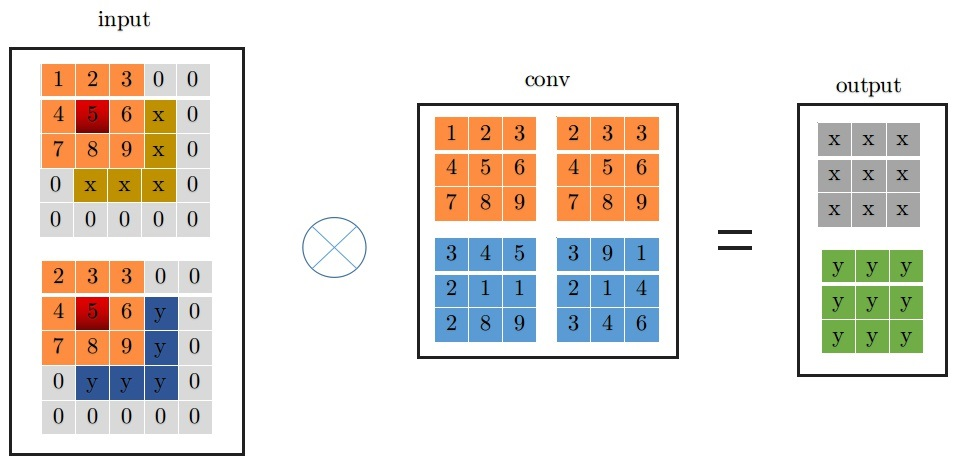
\includegraphics[width=0.8\textwidth]{fuse31_1.jpg}	%\vspace{-1.0em}
    \caption{Conv3*3卷积运算}
    \label{fig:fuse31-1} %\vspace{-0.8em}
\end{figure}

\begin{figure}[]
    \centering
    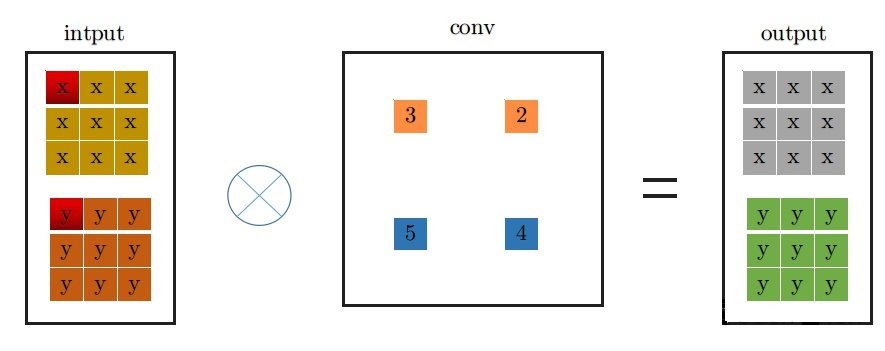
\includegraphics[width=0.8\textwidth]{fuse31_2.jpg}	%\vspace{-1.0em}
    \caption{Conv1*1卷积运算}
    \label{fig:fuse31-2} %\vspace{-0.8em}
\end{figure}

\begin{figure}[]
    \centering
    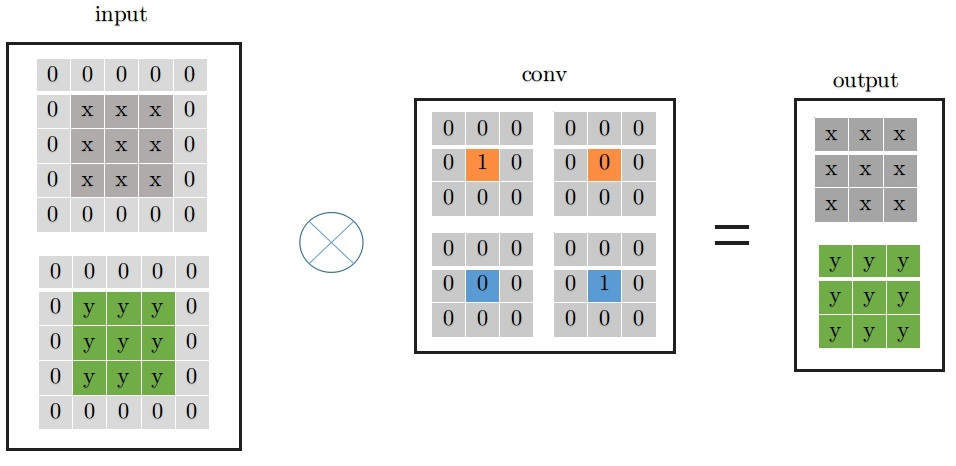
\includegraphics[width=0.8\textwidth]{fuse31_3.jpg}	%\vspace{-1.0em}
    \caption{Conv3*3 和 Conv1*1合并步骤3}
    \label{fig:fuse31-3} %\vspace{-0.8em}
\end{figure}

为了详细说明,假设输入特征图特征图尺寸为(1, 2, 3, 3),输出特征图尺寸与输入特征图尺寸相同,且stride=1,如图~\ref{fig:fuse31-1},展示是Conv3*3的卷及过程:

Conv3*3卷积由上图所示,首先将特征图进行 $pad=kernel_size//2$,然后从上图左上角红色为止做卷积运算,最终得到右边output输出。如图~\ref{fig:fuse31-2}是Conv1*1卷积过程:

同理,Conv1*1跟Conv3*3卷积过程一样,从上图中左边input中红色位置开始进行卷积,得到右边的输出,观察Conv1*1和Conv3*3的卷积过程,从红色起点位置开始,走过相同的计算路径,因此,将Conv1*1跟Conv3*3进行融合,只需要将Conv1*1卷积核padding成Conv3*3的形式,然后于Conv3*3相加,再与特征图做卷积(这里依据卷积的可加性原理)即可,也就是Conv1*1的卷积过程变成如下图~\ref{fig:fuse31-3}形式:


\subsubsection{与identity层等效的卷积层表示}

\begin{figure}[]
    \centering
    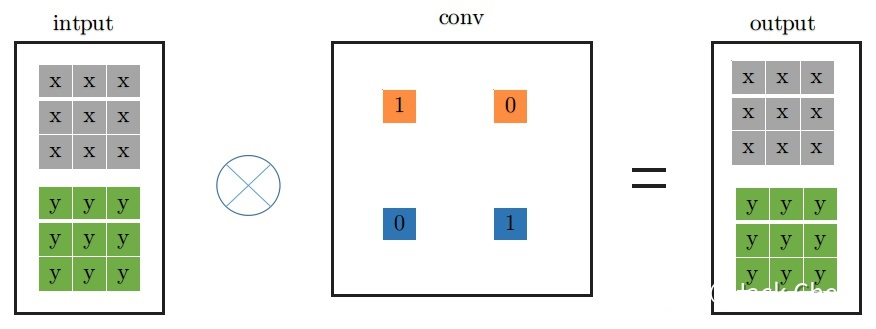
\includegraphics[width=0.8\textwidth]{fuse31_4.jpg}	%\vspace{-1.0em}
    \caption{identity层的Conv1*1表示}
    \label{fig:fuse31-4} %\vspace{-0.8em}
\end{figure}

\begin{figure}[]
    \centering
    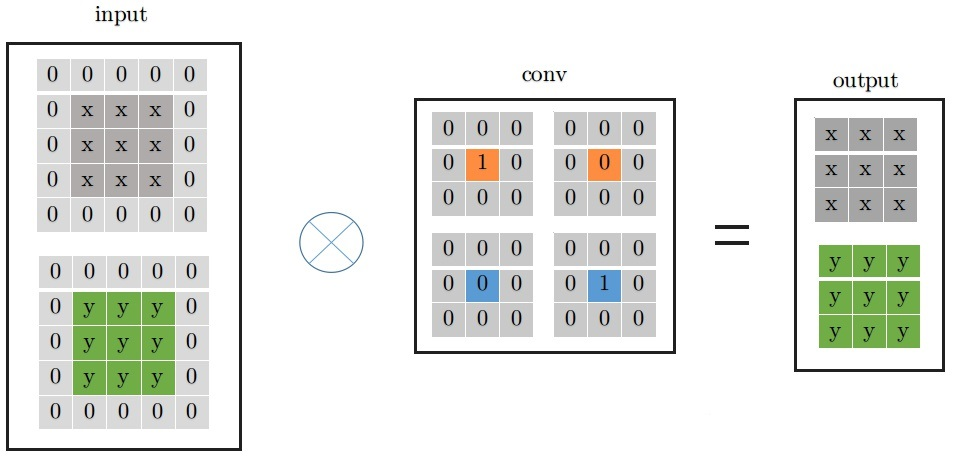
\includegraphics[width=0.8\textwidth]{fuse31_5.jpg}	%\vspace{-1.0em}
    \caption{identity层的Conv3*3表示}
    \label{fig:fuse31-5} %\vspace{-0.8em}
\end{figure}

identity层就是输入等于输出,即input中每个通道每个元素直接输出到output中对应的通道,即相当于值为1的深度可分离卷积,使用普通卷积表示为单位矩阵,因此,identity可以等效成如下图~\ref{fig:fuse31-4}的Conv1*1的卷积形式:

从上面的分析,我们进一步可以将identity -> Conv1*1 -> Conv3*3的形式,如下图~\ref{fig:fuse31-5}所示:

\subsubsection{Conv1*1、Conv3*3与identity层融合}

如图~\ref{fig:fuseall}将Conv1*1与identity都表示为Conv3*3形式,吸收BN层,然后线性可加:

\begin{figure}[]
    \centering
    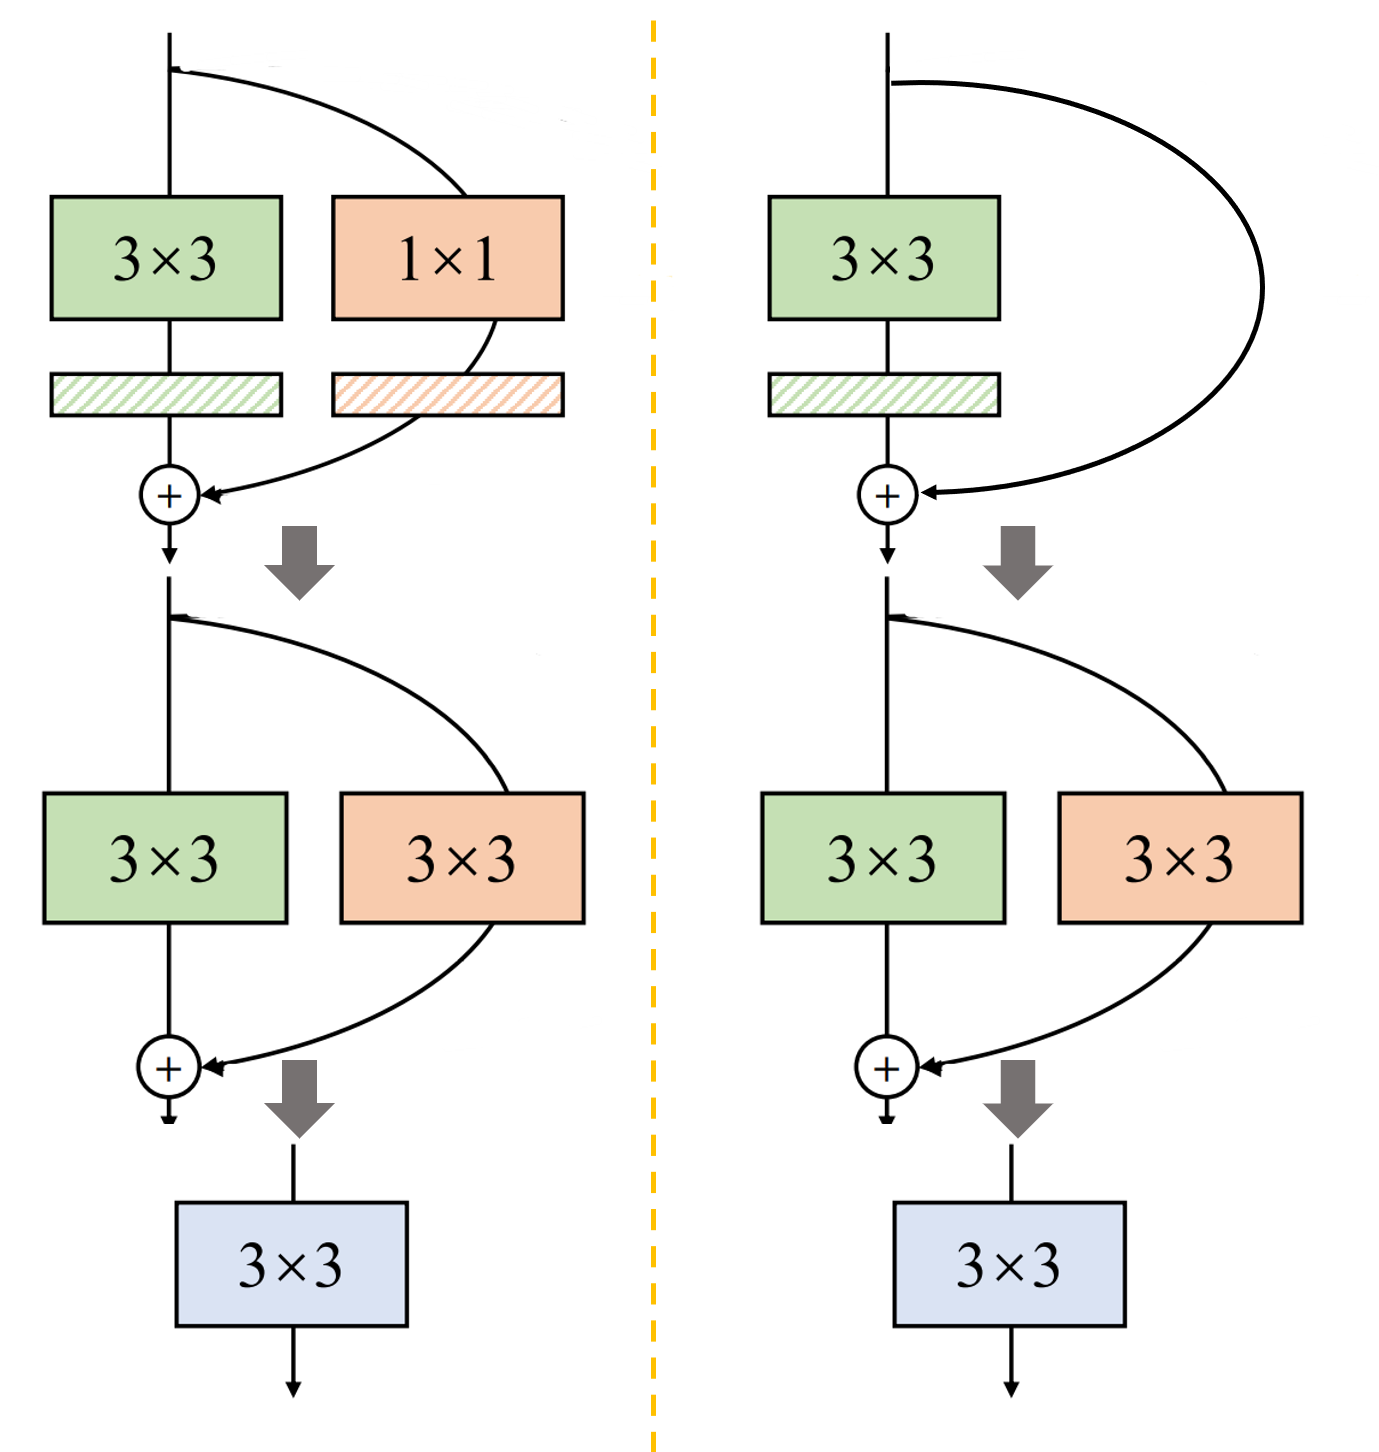
\includegraphics[width=0.8\textwidth]{fuseall.png}	%\vspace{-1.0em}
    \caption{Conv1*1、Conv3*3与identity层融合}
    \label{fig:fuseall} %\vspace{-0.8em}
\end{figure}

\section{实验结果与分析}

在本节中,我们比较了融合分支后的ResNet网络在ImageNet上的基线的推理性能。

\subsection{实验环境设置}

实验使用简单数据增强后的ImageNet数据集,训练120个周期,推理批量尺寸(batchsize)为128,速度单位为示例/秒,在1080Ti上进行32位浮点推理运算。

\subsection{实验结果}

表~\ref{tab:testresult}为在1080ti上的测试结果,本次测试将分支融合部署的ResNet18、ResNet34、ResNet50、ResNet101与其原始模型进行对比,实验表明,我们的分支融合方法效果非常不错。在同样的训练条件下,分支融合部署的网络在精度与速度方面都超过了对应的原始网络。

\begin{table}[]
    \centering
    \caption{ImageNet上训练结果对比}
    \label{tab:testresult} %\vspace{-0.8em}
    \begin{tabular}{lll}
    \hline
    模型                  & Top1准确率        & 速度            \\ \hline
    ResNet18            & 71.16          & 2442          \\
    \textbf{ResNet18*}  & \textbf{72.41} & \textbf{3256} \\ \hline
    ResNet34            & 74.17          & 1419          \\
    \textbf{ResNet34*}  & \textbf{74.46} & \textbf{2339} \\ \hline
    ResNet50            & 76.31          & 719           \\
    \textbf{ResNet50*}  & \textbf{77.78} & \textbf{792}  \\ \hline
    ResNet101           & 77.21          & 430           \\
    \textbf{ResNet101*} & \textbf{78.78} & \textbf{460} 
    \end{tabular}
\end{table}



\section{本章小结}

借助重参数化和辅助训练思想,从这个角度入手,本章提出了网络分支融合部署方法,优化部署时模型推理精度和效率。通过融合多分支结构,辅以知识蒸馏训练,提高模型部署时推理精度和运行效率。首先,讨论了到线性网络结构和多分支网络结构各自的优点和局限性,其次通过微调ResNet网络结构,解耦网络的训练和部署,在训练时使用多分支网络结构,在部署时将其转化为线性网络结构,同时利用了线性网络和多分支网络的优点而规避它们的缺点,最终获得在速度和精度两方面的性能提升。



